\documentclass[12pt,titlepage]{article}
\usepackage[margin=1.25in]{geometry}
\usepackage{graphicx,amsmath,blindtext,tikz}

%% Variables definition
\newcommand{\vSubject}{Basic Programming}
\newcommand{\vSubtitle}{Assignment 10 Loops and Arrays}
\newcommand{\vName}{Dicha Zelianivan Arkana}
\newcommand{\vNIM}{2241720002}
\newcommand{\vClass}{1i}
\newcommand{\vDepartment}{Information Technology}
\newcommand{\vStudyProgram}{D4 Informatics Engineering}

%% [START] Tikz related stuff
\usepackage{tikz}
\usetikzlibrary{svg.path,calc,shapes.geometric,shapes.misc}
\tikzstyle{terminator} = [rectangle, draw, text centered, rounded corners = 1em, minimum height=2em]
\tikzstyle{preparation} = [chamfered rectangle, chamfered rectangle sep=0.75em, draw, text centered, minimum height = 2em]
\tikzstyle{process} = [rectangle, draw, text centered, minimum height=2em]
\tikzstyle{decision} = [diamond, aspect=2, draw, text centered, minimum height=2em]
\tikzstyle{data}=[trapezium, draw, text centered, trapezium left angle=60, trapezium right angle=120, minimum height=2em]
\tikzstyle{connector} = [line width=0.25mm,->]
%% [END] Tikz related stuff

%% [START] Fancy header related stuff
\usepackage{fancyhdr}
\pagestyle{fancy}
\setlength{\headheight}{15pt} % compensate fancyhdr style
\fancyhead{}
\fancyfoot{}
\fancyfoot[L]{\thepage}
\fancyfoot[R]{\textit{\vSubject - \vSubtitle}}
\renewcommand{\footrulewidth}{0.4pt}% default is 0pt, overline for footer
%% [END] Fancy header related stuff

%% [START] Custom tabular command related stuff
\usepackage{tabularx}
\newcommand{\details}[2]{
    #1 & #2  \\
}
%% [END] Custom tabular command related stuff

%% [START] Figure related stuff
\newcommand{\image}[3][1]{
    \begin{figure}[h]
        \centering
        \includegraphics[#1]{#2}
        \caption{#3}
        \label{#3}
    \end{figure}
}
%% [END] Figure related stuff

\begin{document}
\begin{titlepage}
    \centering
    \vfill
    {\bfseries\LARGE
        \vSubject\\
        \vskip0.25cm
        \vSubtitle
    }
    \vfill
    \includegraphics[width=6cm]{images/polinema-logo.png}
    \vfill
    {
        \textbf{Name}\\
        \vName\\
        \vskip0.5cm
        \textbf{NIM}\\
        \vNIM\\
        \vskip0.5cm
        \textbf{Class}\\
        \vClass\\
        \vskip0.5cm
        \textbf{Department}\\
        \vDepartment\\
        \vskip0.5cm
        \textbf{Study Program}\\
        \vStudyProgram
    }
\end{titlepage}

\section*{Assignment}
\subsubsection*{1. Create a flowchart of variable array filling with 50 elements length using looping!}
\begin{center}
    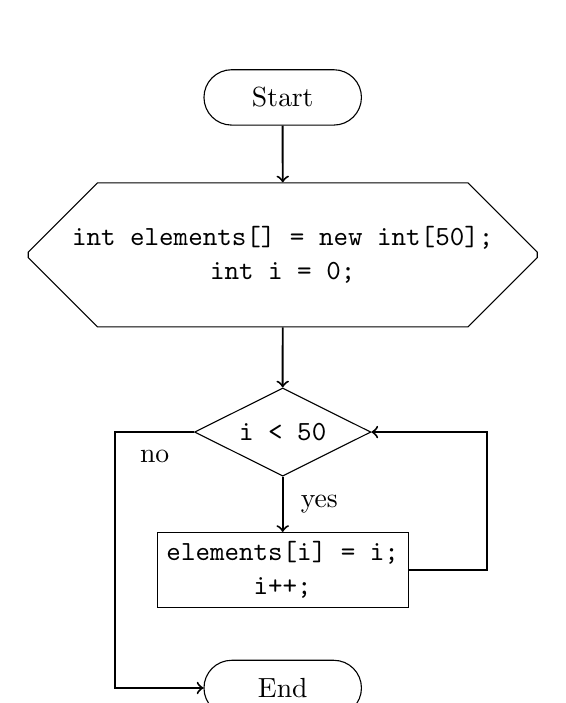
\begin{tikzpicture}
        \node (start) [terminator, align=center, minimum width=2cm, minimum height=2em] {Start};
        \node (prep) [preparation, below of = start, yshift=-1cm, align = center, chamfered rectangle sep=1.25em] {
            \texttt{int elements[] = new int[50];}\\
            \texttt{int i = 0;}
        };
        \node (cond) [decision, below of = prep, yshift=-1.25cm] {\texttt{i < 50}};
        \node (process) [process, below of = cond, yshift=-7.5mm, align=center] {
            \texttt{elements[i] = i;}\\
            \texttt{i++;}
        };
        \node (end) [terminator, below of = process, align=center, minimum width=2cm, minimum height=2em, yshift=-5mm] {End};
        \draw [connector] (start) -- (prep);
        \draw [connector] (prep) -- (cond);
        \draw [connector] (cond) -- node[right=1mm] {yes} (process);
        \draw [connector] (process.east) -- ($(process.east)+(1cm,0)$) |- (cond.east);
        \draw [connector] (cond.west) -- node[below=1mm] {no} ($(cond.west)-(1cm,0)$) |- (end.west);
    \end{tikzpicture}
\end{center}
\pagebreak
\subsubsection*{2. Create a flowchart to fill array elements with 5 elements, then display the contents of array in reverse order!}
\begin{center}
    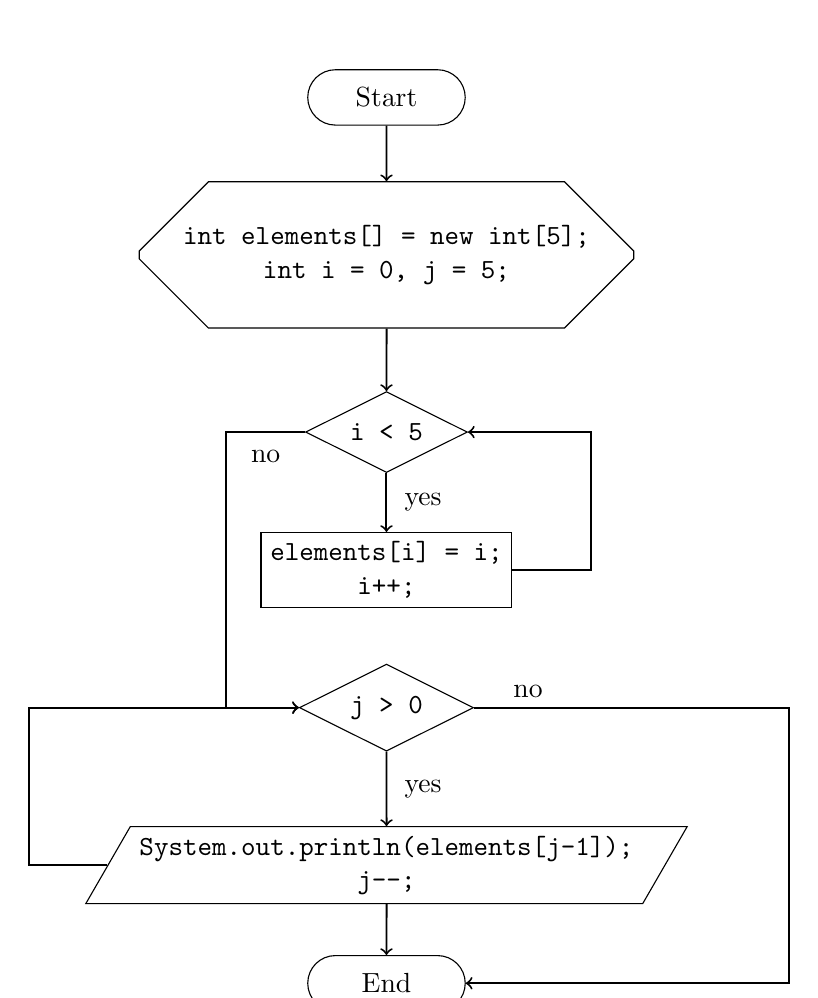
\begin{tikzpicture}
        \node (start) [terminator, align=center, minimum width=2cm, minimum height=2em] {Start};
        \node (prep) [preparation, below of = start, yshift=-1cm, align = center, chamfered rectangle sep=1.25em] {
            \texttt{int elements[] = new int[5];}\\
            \texttt{int i = 0, j = 5;}
        };
        \node (cond) [decision, below of = prep, yshift=-1.25cm] {\texttt{i < 5}};
        \node (process) [process, below of = cond, yshift=-7.5mm, align=center] {
            \texttt{elements[i] = i;}\\
            \texttt{i++;}
        };
        \node (print-cond) [decision, below of = process, yshift=-7.5mm] {\texttt{j > 0}};
        \node (print) [data, below of = print-cond, yshift=-1cm,align=center] {
            \texttt{System.out.println(elements[j-1]);}\\
            \texttt{j--;}
        };
        \node (end) [terminator, below of = print, align=center, minimum width=2cm, minimum height=2em, yshift=-5mm] {End};
        \draw [connector] (start) -- (prep);
        \draw [connector] (prep) -- (cond);
        \draw [connector] (cond) -- node[right=1mm] {yes} (process);
        \draw [connector] (process.east) -- ($(process.east)+(1cm,0)$) |- (cond.east);
        \draw [connector] (cond.west) -- node[below=1mm] {no} ($(cond.west)-(1cm,0)$) |- (print-cond.west);
        \draw [connector] (print-cond) -- node[right=1mm] {yes} (print);
        \draw [connector] (print-cond.east) -- node[above=2mm,left=1cm] {no} ($(print-cond.east)+(4cm,0)$) |- (end.east);
        \draw [connector] (print.west) -- ($(print.west)-(1cm,0)$) |- (print-cond);
        \draw [connector] (print) -- (end);
    \end{tikzpicture}
\end{center}

\end{document}

